\documentclass[a4paper,12pt]{article}

% Idioma y codificación
\usepackage[spanish]{babel}
\usepackage[utf8]{inputenc}
\usepackage[T1]{fontenc}

% Matemáticas y símbolos
\usepackage{amsmath, amssymb}

% Algoritmos (pseudocódigo sencillo)
\usepackage[ruled,vlined]{algorithm2e}

% Otros paquetes útiles
\usepackage{graphicx}
\usepackage{hyperref}
\usepackage{float}

\begin{document}

\section{Comparación de Modelos Supervisados}

\subsection{Descripción del problema}
El objetivo de este taller es implementar un flujo de trabajo completo de aprendizaje supervisado para comparar el desempeño de tres clasificadores: \textbf{Random Forest}, \textbf{kNN} y \textbf{SVM}.  

El análisis se realizó sobre dos conjuntos de datos clásicos: \textbf{Iris}, que contiene 150 muestras con 4 características numéricas y 3 clases balanceadas; y \textbf{Diabetes}, que incluye 768 muestras con 8 atributos clínicos y una variable binaria ($0$: No Diabetes, $1$: Diabetes), la cual presenta desbalance entre clases.  

La importancia de este problema radica en que permite observar cómo los modelos se comportan en escenarios distintos: uno balanceado y de baja dimensionalidad (Iris), y otro más complejo y desbalanceado (Diabetes). El resultado esperado es evidenciar diferencias en precisión, robustez y sensibilidad de cada algoritmo, así como la relevancia del preprocesamiento.

\subsection{Método de solución}
Para abordar el problema, se diseñó un flujo de trabajo supervisado utilizando la librería \texttt{scikit-learn} en Python. El procedimiento consistió en:  

\begin{itemize}
    \item División estratificada de los datos en entrenamiento (80\%) y prueba (20\%).
    \item Preprocesamiento con \texttt{StandardScaler} en los modelos sensibles a la escala (kNN y SVM).
    \item Entrenamiento de los modelos: Random Forest, kNN y SVM.
    \item Validación cruzada 5-fold para estimar desempeño promedio.
    \item Evaluación en el conjunto de prueba con métricas (\textit{accuracy}, \textit{precision}, \textit{recall}, \textit{f1-score}) y matrices de confusión.
    \item Comparación de resultados para determinar fortalezas y limitaciones de cada algoritmo.
\end{itemize}

Los datos empleados fueron:
\begin{itemize}
    \item \textbf{Iris}: 150 instancias con 4 características; 3 clases balanceadas.
    \item \textbf{Diabetes  }: 768 instancias con 8 características clínicas; variable de salida binaria desbalanceada.
\end{itemize}

El pseudocódigo general de este procedimiento se presenta en el Algoritmo~\ref{alg:workflow}.  

\vspace{0.5cm}

\begin{algorithm}[H]
\caption{Flujo de trabajo supervisado}
\label{alg:workflow}
\SetKwInput{KwIn}{Entrada}
\SetKwInput{KwOut}{Salida}
\KwIn{Dataset $D$, Modelos $M=\{\text{RF}, \text{kNN}, \text{SVM}\}$}
\KwOut{Métricas y matrices de confusión}

Dividir $D$ en train y test (80/20, estratificado)\;
Para cada modelo $m \in M$ hacer:\;
\Indp
    Preprocesar datos si es necesario (escalado)\;
    Entrenar $m$ con los datos de entrenamiento\;
    Validar desempeño con \texttt{cross-validation} (cv=5)\;
    Evaluar $m$ con los datos de prueba\;
    Calcular métricas (accuracy, precision, recall, f1)\;
    Generar matriz de confusión\;
\Indm
Comparar resultados y seleccionar el modelo más robusto\;
\end{algorithm}

\subsection{Resultados}
La ejecución del código se realizó en Python, utilizando los archivos \texttt{iris.csv} y \texttt{diabetes.csv} como conjuntos de datos de entrada.  
El flujo de trabajo descrito permitió entrenar y evaluar los tres modelos (\textbf{Random Forest}, \textbf{kNN}, \textbf{SVM}) bajo un esquema de división estratificada (80/20) y validación cruzada 5-fold.  

Los principales resultados obtenidos se resumen en la Tabla~\ref{tab:resultados}, donde se reportan los valores promedio de \textit{accuracy} para cada combinación de dataset y modelo.  

\begin{table}[H]
    \centering
    \caption{Resultados de \textit{accuracy} promedio por modelo y dataset.}
    \label{tab:resultados}
    \begin{tabular}{|c|c|c|}
        \hline
        \textbf{Modelo} & \textbf{Iris (Accuracy)} & \textbf{Diabetes (Accuracy)} \\ \hline
        Random Forest & 0.9667 & 0.7670 \\ \hline
        kNN           & 0.9733 & 0.7240 \\ \hline
        SVM           & 0.9667 & 0.7591 \\ \hline
    \end{tabular}
\end{table}

Además de las métricas globales, se generaron matrices de confusión que permiten analizar los errores de clasificación.  
A continuación, se presentan las gráficas correspondientes para cada modelo y dataset:

\begin{figure}[H]
    \centering
    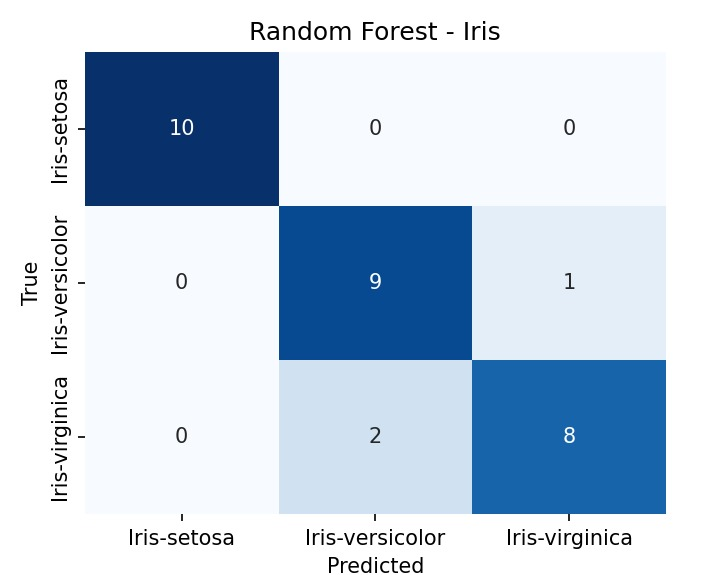
\includegraphics[width=0.6\textwidth]{figuras/iris_rf.png}
    \caption{Matriz de confusión del modelo Random Forest en el dataset Iris.}
    \label{fig:iris_rf}
\end{figure}

\begin{figure}[H]
    \centering
    
    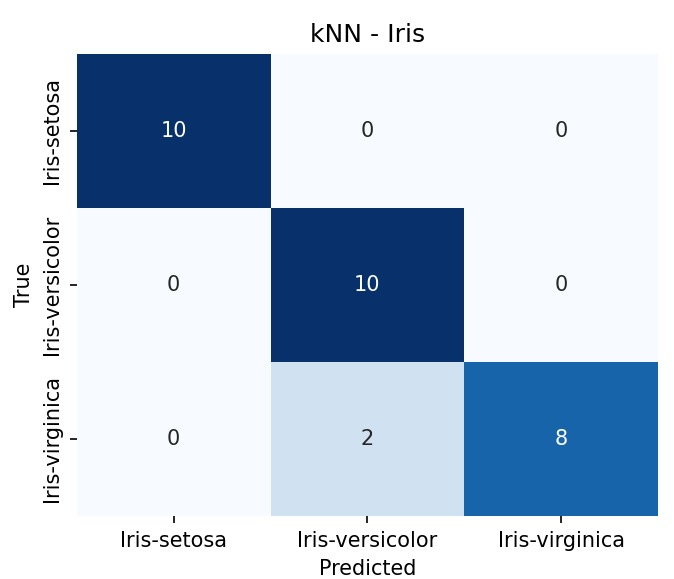
\includegraphics[width=0.6\textwidth]{figuras/iris_knn.png}
    \caption{Matriz de confusión del modelo kNN en el dataset Iris.}
    \label{fig:iris_knn}
\end{figure}

\begin{figure}[H]
    \centering
    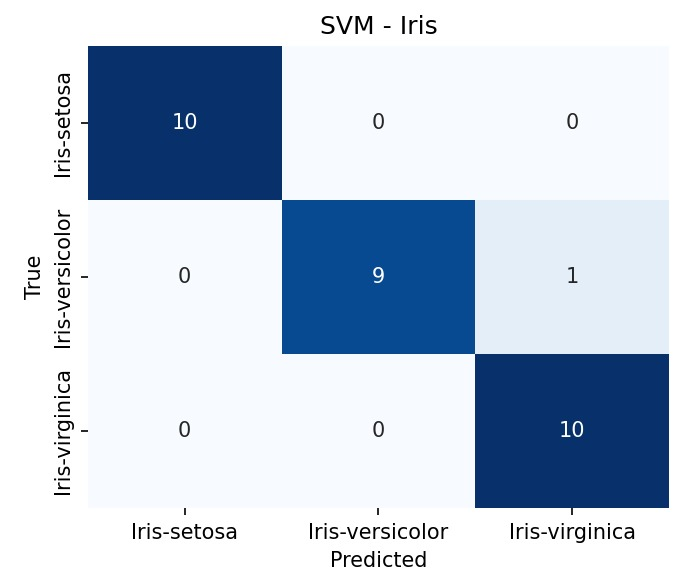
\includegraphics[width=0.6\textwidth]{figuras/iris_svm.png}
    \caption{Matriz de confusión del modelo SVM en el dataset Iris.}
    \label{fig:iris_svm}
\end{figure}

\begin{figure}[H]
    \centering
    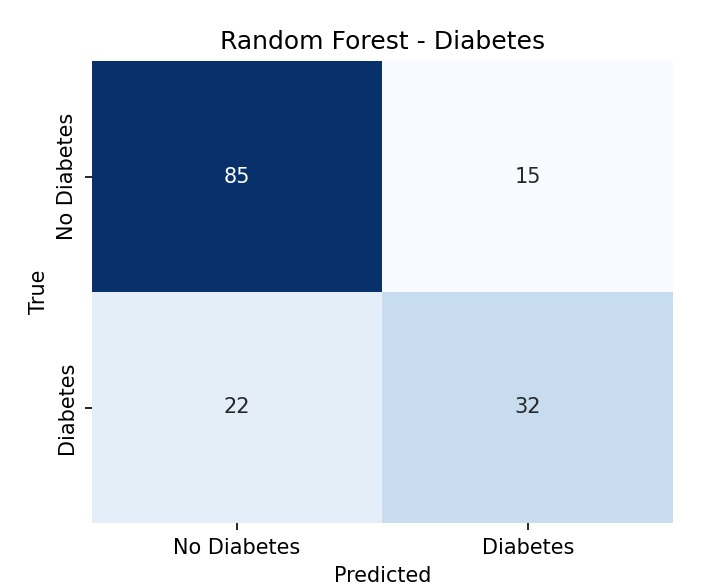
\includegraphics[width=0.6\textwidth]{figuras/diabetes_rf.png}
    \caption{Matriz de confusión del modelo Random Forest en el dataset Diabetes.}
    \label{fig:db_rf}
\end{figure}

\begin{figure}[H]
    \centering
    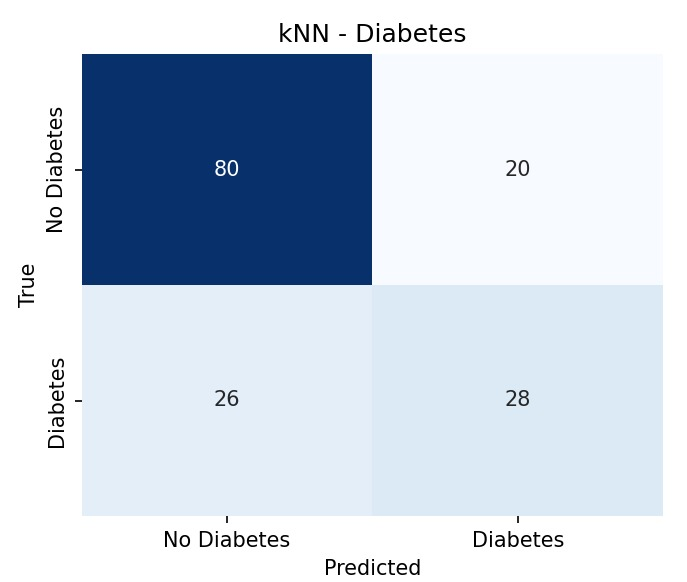
\includegraphics[width=0.6\textwidth]{figuras/diabetes_knn.png}
    \caption{Matriz de confusión del modelo kNN en el dataset Diabetes.}
    \label{fig:db_knn}
\end{figure}

\begin{figure}[H]
    \centering
    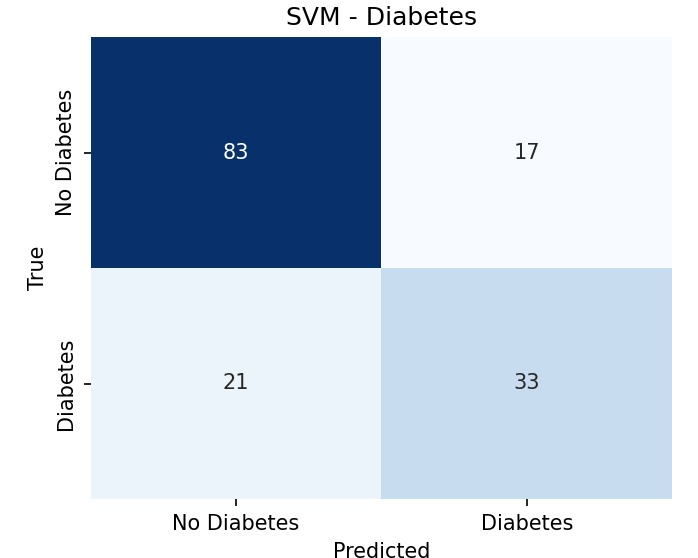
\includegraphics[width=0.6\textwidth]{figuras/diabetes_svm.png}
    \caption{Matriz de confusión del modelo SVM en el dataset Diabetes.}
    \label{fig:db_svm}
\end{figure}

En términos generales, los modelos alcanzaron un desempeño cercano al 97\% en el dataset Iris, mientras que en el dataset Diabetes el rendimiento fue menor (70–77\%).  
Estos resultados muestran la diferencia en complejidad entre ambos problemas y reflejan la importancia del preprocesamiento y la elección de hiperparámetros en kNN y SVM.

\subsection{Discusión}
Los resultados muestran una clara diferencia entre los dos problemas analizados. 
En el dataset \textbf{Iris}, los tres modelos alcanzaron desempeños muy altos 
(accuracy cercano al 97\%), lo cual refleja la simplicidad del problema y el 
equilibrio en la distribución de clases.  

En contraste, en el dataset \textbf{Diabetes}, los desempeños se ubicaron entre 
70\% y 77\%, evidenciando la mayor dificultad asociada a datos desbalanceados 
y con mayor complejidad clínica. Esto resalta la importancia de aplicar técnicas 
de preprocesamiento y, en algunos casos, de considerar ajustes como balanceo de 
clases o selección de atributos relevantes.  

Comparando los algoritmos, \textbf{Random Forest} mostró ser el más robusto al 
mantener un rendimiento competitivo en ambos datasets, mientras que kNN y SVM 
se vieron más afectados por el desbalance y la necesidad de un escalado adecuado.  

En síntesis, se puede concluir que el tipo de dataset influye significativamente 
en el desempeño de los modelos, y que la elección del algoritmo debe considerar 
las características propias del problema a resolver.

\subsection{Conclusiones}
El presente trabajo permitió comparar el desempeño de tres algoritmos de 
clasificación supervisada (\textbf{Random Forest}, \textbf{kNN} y \textbf{SVM}) 
sobre dos conjuntos de datos con características contrastantes: uno balanceado 
y de baja dimensionalidad (\textit{Iris}) y otro más complejo y desbalanceado 
(\textit{Diabetes}).  

De los resultados obtenidos se concluye que:  
\begin{itemize}
    \item Los modelos alcanzan altos niveles de \textit{accuracy} en el dataset 
    Iris (cercanos al 97\%), lo que confirma que se trata de un problema sencillo 
    y bien estructurado.
    \item En el dataset Diabetes, los valores de desempeño fueron menores (70--77\%), 
    lo que refleja la dificultad de trabajar con datos clínicos más ruidosos y 
    desbalanceados.
    \item \textbf{Random Forest} resultó ser el modelo más robusto, manteniendo 
    un buen desempeño en ambos escenarios sin requerir un preprocesamiento 
    intensivo.
    \item Algoritmos como kNN y SVM demostraron sensibilidad a la escala de las 
    variables y al desbalance de clases, lo que resalta la importancia de aplicar 
    técnicas de normalización y ajuste de hiperparámetros.
\end{itemize}

Cabe resaltar que, en el caso del dataset de Diabetes, métricas como el \textit{recall} de la clase positiva (diabéticos) son especialmente relevantes, ya que en un contexto clínico un falso negativo puede tener consecuencias más graves que un falso positivo.

En términos generales, se evidencia que la elección del algoritmo depende en 
gran medida de las características del conjunto de datos. Asimismo, se destaca 
la relevancia de estrategias de preprocesamiento y validación cruzada para 
garantizar resultados más confiables y generalizables.


\end{document}

